% -------------------
% Preamble - Packages and Document Setup
% -------------------
\documentclass[12pt, a4paper]{article}

% --- PACKAGES ---
\usepackage[utf8]{inputenc}
\usepackage[T1]{fontenc}
\usepackage{amsmath}
\usepackage{amssymb}
\usepackage{graphicx}
\usepackage{geometry}
\usepackage{authblk}
\usepackage{abstract}
\usepackage{times}
\usepackage{natbib}
\usepackage{setspace}
\usepackage{fancyhdr}
\usepackage{lastpage}
\usepackage[hidelinks]{hyperref}
\usepackage{booktabs}
\usepackage[font=small, labelfont=bf, margin=1cm]{caption}
%\usepackage[font={small, it}, labelfont=bf, margin=1cm]{caption}

% --- GEOMETRY AND LAYOUT ---
\geometry{
  a4paper,
  margin=1in,
  top=0.8in,
  bottom=1in
}
\setstretch{1.19} % Subtle visual compression (standard onehalfspacing is ~1.24)
\setlength{\parskip}{0.2em} % Slightly tighter paragraph spacing

\title{
    \Large \textbf{The Language State Machine (LSM) Architecture} \\
    \large A Reference Framework for Stateful AI Narrative Orchestration \\
    \vspace{1em}
    \small Protocol ID: \texttt{MMG-LSM-1.0} \\
    \small \textbf{Status:} \textit{Systems Specification for Persistent Generative Realities}
}


\author{\vspace{0.8em}Djeff Bee\thanks{Correspondence: \href{mailto:info@meaningfulness.com.au}{info@meaningfulness.com.au}}}
\affil{\vspace{-0.5em}\textit{Principal Architect, Meaningfulness Media Group}}
\date{\vspace{-0.5em}May 25, 2026}

% -------------------
% Front Matter - Title, Abstract, and Keywords
% -------------------
\begin{document}

\maketitle
\vspace{-2em}

\thispagestyle{fancy}
\fancyhf{}
\renewcommand{\headrulewidth}{0pt}
\cfoot{
    \footnotesize
    Copyright \copyright\ 2026 Meaningfulness Media Group. \\
    This paper is licensed under \href{https://creativecommons.org/licenses/by/4.0/}{CC BY 4.0}. \\
    The TomeWeaver reference implementation is licensed separately (Polyform Noncommercial 1.0.0).
}

\begin{abstract}
\noindent
Large Language Models (LLMs) are fundamentally stateless functions. When applied to long-form interactive fiction, relying exclusively on the model's context window for state management leads to a structural failure we term \textit{Contextual Amnesia}---the inevitable decay of established world facts over long sessions. This paper proposes the Language State Machine (LSM), a software architecture that decouples generative prose from absolute world state. By treating the story as an indexed database rather than a chat transcript, we constrain the LLM to act strictly as a rendering engine. We introduce TomeWeaver as a reference implementation, detailing its six-layer KERNEL architecture, its dual-tiered Retrieval-Augmented Generation (RAG) memory system, and its approach to non-destructive timeline editing. Ultimately, we argue that narrative coherence is not a prompting problem, but an architectural one: the LLM must be treated not as an authoritative record of reality, but as a \textbf{probabilistic coprocessor} orchestrated by a deterministic state machine, preventing unvalidated structural corruption while keeping narrative truth under the Director's active control.
\end{abstract}

\vspace{0.5em}
\noindent\textbf{Keywords:} Language State Machines, Retrieval-Augmented Generation, Interactive Fiction, LLM Systems Design, State Management.

\vspace{1em}
\noindent
\fbox{
    \parbox{\textwidth}{
        \centering
        \textbf{Reference Implementation} \\
        \vspace{0.5em}
        \begin{tabular}{r l}
            \textbf{Engine:} & \textit{TomeWeaver} (\href{https://github.com/MeaningfulnessMediaGroup/TomeWeaver}{github.com/MeaningfulnessMediaGroup/TomeWeaver}) \\
            \textbf{API:} & Headless Python Library Facade with pytest coverage. \\
        \end{tabular}
    }
}

% --- HEADER SETTINGS ---
\newpage
\pagestyle{fancy}
\thispagestyle{fancy}
\fancyhf{}
\renewcommand{\sectionmark}[1]{\markboth{#1}{}}
\renewcommand{\subsectionmark}[1]{}
\fancyhead[L]{\footnotesize MMG-LSM-1.0}
\fancyhead[R]{\footnotesize \nouppercase{\leftmark}}
\cfoot{
    Page \thepage\ of \pageref{LastPage}
}
\renewcommand{\headrulewidth}{0.4pt}



% -------------------
% Section 1 - Introduction: The End of the Infinite Scroll
% -------------------
\section{Introduction: The End of the Infinite Scroll}
\label{sec:intro}

If you have spent any serious time trying to run a long RPG campaign through a Large Language Model, you know exactly how the illusion dies. It doesn't throw a fatal exception. It just quietly loses its mind.

For the first twenty turns, the experience feels like magic. You type an action, the model responds with brilliant prose, and the world feels alive. Then you hit turn forty. The tavern you explicitly burned to the ground in chapter one is suddenly open for business. Your protagonist's broken arm heals itself without a word. The villain forgets your name. Items simply wander out of the narrative.

I call this Contextual Amnesia. The AI industry keeps trying to patch this by throwing hardware at the problem, bragging about million-token context windows and infinite scroll interfaces. But stuffing a massive chat transcript into a prompt isn't a memory architecture. It is a hoarding problem. 

Finite context windows, unstructured chat transcripts, and overwrite-based editing make the past incredibly expensive to retrieve and miserable to revise. Even if you have the API budget to pass a hundred thousand words into a model on every single turn, you run headfirst into attention dilution; research demonstrates that LLMs reliably fail to retrieve facts buried in the middle of long contexts \citep{liu2023lost}. The model gets lost in the middle of its own history.

This paper is not about how to write a more desperate, thousand-word system prompt. It is about recognizing that the "chatbot" paradigm is fundamentally the wrong software architecture for long-form interactive fiction.

The architectural question we have to answer is blunt: \textit{where should narrative state live, and who is actually allowed to mutate it while the LLM is generating?}

\subsection{The Language State Machine}

The solution is to stop treating the story as a disposable chat log and start treating it as a state machine. 

I propose the \textbf{Language State Machine (LSM)} architecture. It is a strict decoupling of generative prose from absolute world state. The LLM shouldn't own your reality. It should simply be the rendering engine that paints it. 

To prove this is not just academic theory, I built \textbf{TomeWeaver}. It is a working, open-source reference implementation of the LSM pattern. It utilizes a layered architecture to physically isolate the LLM from the actual game state, wrapping the model in deterministic Python logic that prevents hallucinated facts from automatically corrupting the ledger. By treating the active turn as a mutable, provisional draft, the system prevents unvalidated structural corruption of the ledger, keeping narrative truth under the Director's active control before any state is permanently committed.

\subsection{Scope and Contributions}

This paper makes three specific contributions to the field of computational narratology:
\begin{enumerate}
    \item It defines the Language State Machine as a reference architecture that any developer can implement in whole or in part. 
    \item It offers the \textbf{KERNEL} decomposition: six inspectable layers of narrative state management that prevent developers from collapsing their architecture back into a monolithic prompt string.
    \item It provides a worked reference implementation (TomeWeaver) complete with on-disk cartridge formats, a headless engine, and automated tests.
\end{enumerate}

To be explicit about the scope of this work: this is a systems design and architecture paper, not an empirical benchmark report. The evaluation metrics proposed in Section \ref{sec:falsifiability} define future comparative work, while TomeWeaver serves as the working reference implementation used to demonstrate the computational feasibility of the pattern.

By decoupling the generative capabilities of the LLM from the storage of reality, this methodology addresses a growing crisis in commercial AI deployment: trust. Systems that cannot be deterministically audited cannot be trusted with persistent data. While current literature heavily focuses on multi-agent debate or chain-of-thought reasoning to improve accuracy from \textit{within} the prompt, we argue that structural scaffolding at the \textit{application layer} yields far more reliable and computationally efficient results. The LSM framework shifts the burden of coherence from the probabilistic model to the deterministic engine.

Although long-form interactive fiction serves as the proving ground for this architecture, the underlying pattern generalizes to any persistent generative simulation where probabilistic outputs must be reconciled with durable state (e.g., multi-agent ecosystems or AI-assisted game engines).

I am not claiming that standard chat interfaces are obsolete for quick improvisational brainstorming, nor am I claiming TomeWeaver guarantees literary greatness. I am claiming that long-form narrative coherence stops being a nightly emergency when state is externalized, scoped, and editable. This is a reusable engineering pattern.



\newpage
% -------------------
% Section 2 - State-Anemic vs. State-Rigorous Design
% -------------------
\section{State-Anemic vs. State-Rigorous Design}
\label{sec:crisis}

\subsection{The Transcript as a False Database}

If you look under the hood of many popular AI storytelling platforms today, you will find they still default to the same underlying abstraction: a linear JSON array of chat-like messages. 

We have taken a user-interface paradigm---the messaging app---and tricked ourselves into believing it is a persistence layer. It is not. When your world state is derived strictly from a linear transcript of prose, your application is structurally brittle. I call these systems \textbf{state-anemic}. In a state-anemic architecture, the authoritative memory of the game is whatever happens to fit inside the prompt payload today.




When you build on top of a state-anemic foundation, you inevitably run into four hard failure modes:

\begin{itemize}
    \item \textbf{The Context Compactor:} As the transcript grows, raw history competes with world lore, entity definitions, and stylistic instructions for prompt space. Something has to give. You end up relying on the model to summarize its own history, which leads to lossy compression. The nuance is squeezed out of the world.
    \item \textbf{Generative Drift:} Because there is no external database validating the AI's output, prose becomes the only source of truth. If the model hallucinates that a character is carrying a pistol instead of a sword, and you don't catch it immediately, that pistol is now officially part of the transcript. The model reads it on the next turn, assumes it is canon, and starts believing its own lies.
    \item \textbf{The Audit Nightmare:} In a state-anemic tool, if you want to know exactly when and why the AI decided a certain faction was hostile to you, your only debugging tool is to manually scroll up and read forty pages of generated text. There is no queryable ledger. The audit cost is linear and entirely manual.
    \item \textbf{Destructive Mutation:} How do you fix a mistake in a chat log? You hit "Regenerate," or you edit the text directly and overwrite what was there. You destroy the previous state. There is no version control, no diffing, and no clear record of what the human authored versus what the machine hallucinated.
\end{itemize}


None of these are LLM failures. They are software engineering failures. We are handing a text-prediction algorithm a massive, unstructured string of text and asking it to perform strict state-management in its latent space. It is the wrong tool for the job.

\newpage
\subsection{The Architectural Pivot}

A \textbf{state-rigorous} system completely inverts this hierarchy. We define a \textbf{state-rigorous system} as one in which authoritative world state is externalized, computationally queryable, and independently validated outside the generative model's context window. In this pattern, the language model is demoted. It is no longer the author of reality; it is merely a rendering engine translating hard data into natural language.

The truth of the world is held externally by the engine---in schemas, chronological ledgers, and compiled memory fragments. 

\begin{table}[h]
\centering
\caption{Design Dimensions (Ideal Types)}
\label{tab:contrast}
\small
\begin{tabular}{@{}p{0.20\textwidth}p{0.36\textwidth}p{0.36\textwidth}@{}}
\toprule
\textbf{Dimension} & \textbf{State-Anemic (Chatbots)} & \textbf{State-Rigorous (LSM)} \\
\midrule
\textbf{Primary Artifact} & Plaintext chat transcript & Cartridge: Schema + Ledger + Memory \\
\textbf{Long Memory} & Context-window stuffing & Compiled RAG + Scoped Injection \\
\textbf{Edit Semantics} & Overwrite / Regenerate & Diffs, Bridges, and Timeline Surgery \\
\textbf{Time Navigation} & Infinite Scroll & Indexed Master Clock + Bookmarks \\
\textbf{Cross-Story Canon} & Manual copy-paste & Scoped shared files (Universes) \\
\textbf{Continuity Authority} & Model hallucination + User recall & Engine commits + Automated audits \\
\textbf{Operator Role} & Prompter & Director / Analyst \\
\bottomrule
\end{tabular}
\end{table}

I want to be clear: state-anemic design is not inherently bad. If you are building a tool for quick improvisational brainstorming, a chat interface is lightweight and frictionless. 

But if you are building an engine for \textit{sustained campaigns}---stories that span hundreds of turns, exportable novels, shared multiverses, and deep narrative mechanics---frictionless chat falls apart. You need rigor. You need an architecture that expects the AI to make mistakes and catches them before they are committed to the hard drive.

\subsection{The Necessity of Structural Scaffolding}

A common counter-argument in the generative AI space is that models will eventually "reason" their way out of hallucination if given enough time and parameter count. This perspective treats coherence as a cognitive goal for the model to achieve. The LSM framework rejects this as an unreliable systems-engineering path. Coherence is not a cognitive task; it is a structural one.

By providing external scaffolding---hardcoded schemas for inventory, sequential master clocks for time, and fidelity-scored ledgers for memory---we relieve the model of the burden of maintaining reality. This allows the prose engine to focus entirely on its greatest strength: linguistic creativity. In this model, the engine's "intellect" is not found in the latent space of the model, but in the structural integrity of the application surrounding it. We move from hoping for a smarter AI to architecting a more durable reality.

This structural scaffolding creates what we term \textbf{Ontological Anchoring}. Every turn is anchored to a specific point in the ledger and a specific set of world rules. Even if the model generates a paragraph that wanders off-course, the anchor remains. The Director can surgically correct the prose without the risk of the model’s error "leaking" into the foundational facts of the world.

\vspace{1cm} 

\begin{figure}[hbt!]
    \centering
    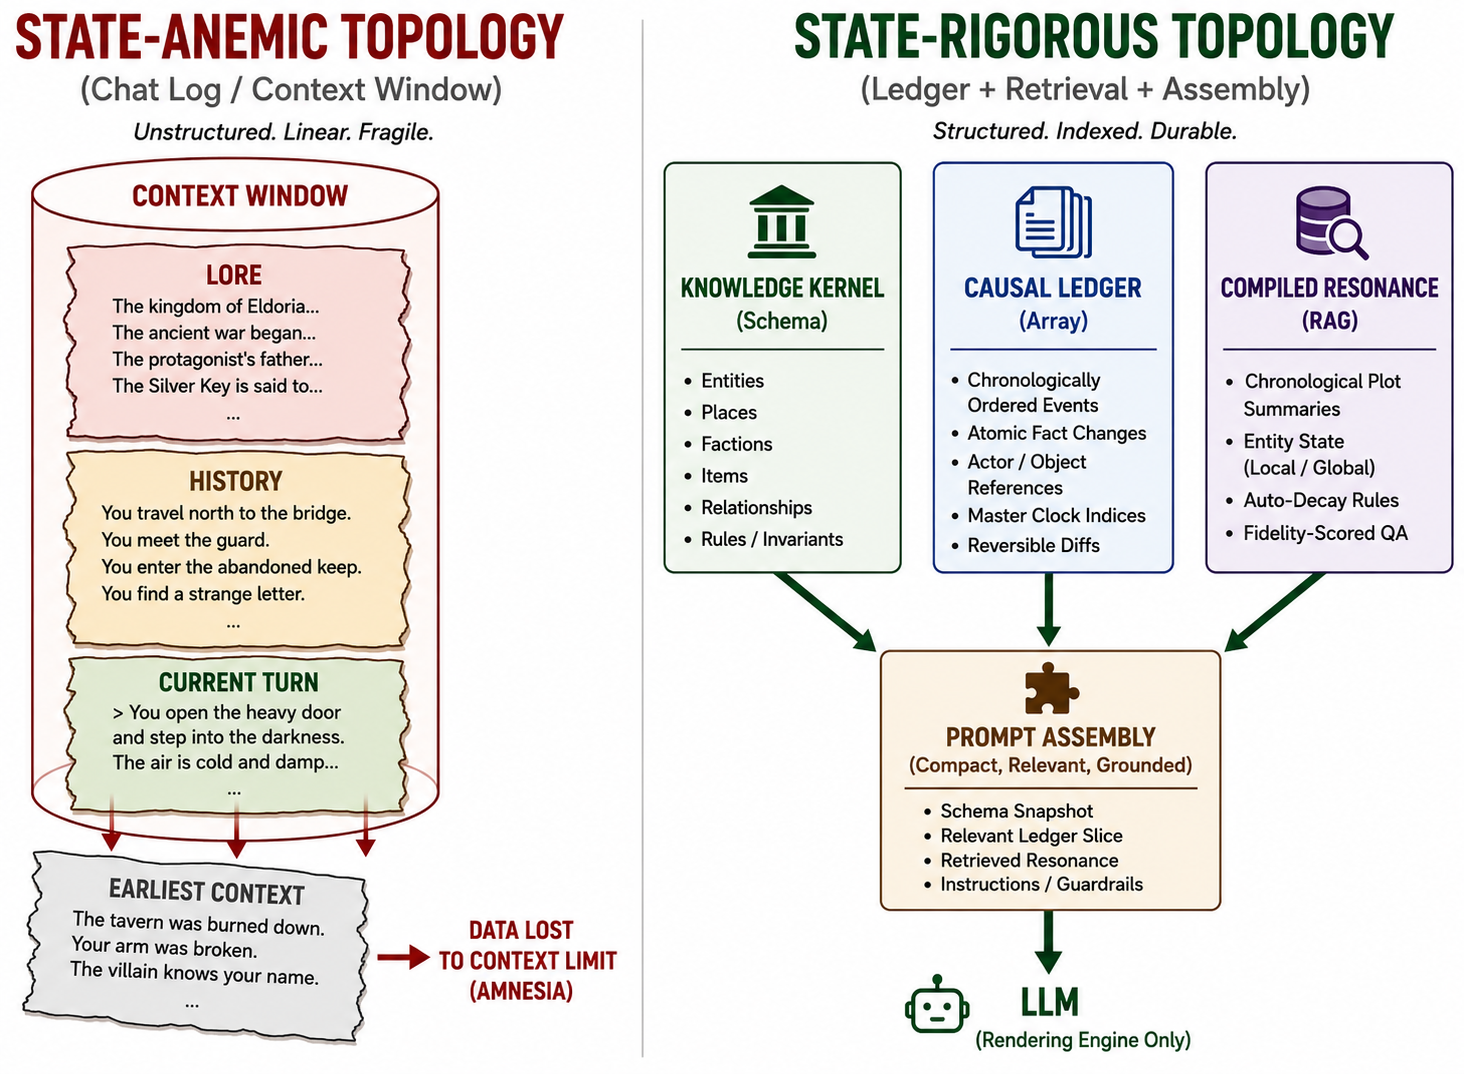
\includegraphics[width=1\textwidth]{images/fig_topology.png}
    \caption{Data topology comparison. State-anemic systems (left) rely on a volatile, linear context window subject to attention dilution and truncation. The LSM architecture (right) compartmentalizes data into discrete, queryable ledgers, assembling context deterministically at runtime.}
    \label{fig:topology}
\end{figure}



\newpage
% -------------------
% Section 3 - Non-Destructive Orchestration
% -------------------
\section{Non-Destructive Orchestration}
\label{sec:principle}

\subsection{The Editing Philosophy}

Every piece of software that allows a user to edit a long, complex document eventually has to define what the word "edit" actually means. In the Chatbot Era, an edit is treated as a localized overwrite. You scrub the text, replace it, and the old reality simply ceases to exist.

When orchestrating a complex, branching narrative, overwrite-based editing is toxic, leading to \textbf{Cumulative Hallucination}. If the model hallucinates a factual error on Turn 10, and the user manually "fixes" the prose without correcting the underlying RAG or ledger state, the system enters an internal contradiction: the model continues to reference the error in its latent memory while the user sees the correction. This destroys forensic traceability. If the narrative derails at Turn 50, tracing the causal error is impossible if the intervening states have been silently overwritten.

TomeWeaver operates on a fundamentally different principle: \textbf{Non-Destructive Orchestration}.

\begin{center}
    \textit{The past is evidence, not draft material. Creative revision must preserve causal traceability.}
\end{center}

To enforce this, the engine relies on a \textbf{Master Clock}---a strict, sequential integer index assigned by the Python backend to every generated turn. We must distinguish between \textit{Latent Time} (the model's unreliable internal perception of event sequence) and \textit{Engine Time} (the deterministic coordinate system of the ledger). LLMs are notoriously incapable of tracking absolute time or counting accurately over long contexts. By externalizing the temporal axis into the Master Clock, the engine guarantees that causality only flows in one direction. This relative temporal coordinate system ensures that every fact, item discovery, or character death is timestamped and, once committed, \textbf{immutable from the perspective of the AI} (the model is physically locked out of altering history, while the human Director retains full administrative editing rights).

Within this model, we introduce the distinction between the \textbf{Provisional Active Turn} and the \textbf{Committed Past}. When the engine generates Turn $N$ (the active turn), it is written to disk for persistence, but it remains in an open, mutable state. Because no downstream decisions depend on it yet, the Director can freely edit, polish, or reroll this active turn without causal consequence. The turn is only "committed" to the immutable past the exact moment the Director submits an action to generate Turn $N+1$. 

To be clear, Non-Destructive Orchestration does not mean "never delete anything." A simulation requires the freedom to prune dead ends. TomeWeaver deletes turns. It merges chapters. It forks entire timelines. However, the architecture demands that these operations be treated as \textbf{named state transitions} rather than text edits.

If you change the timeline, the engine \textbf{deterministically} re-indexes the Master Clock, updates the chapter bounding integers, and invalidates affected RAG summaries. This forces the Director to confront the causal gaps created by the revision. We treat narrative surgery with the same gravity as a database migration. You do not get to silently delete a paragraph and pretend the timeline was always that way; you must explicitly authorize a re-indexing of reality.


\subsection{Putting Theory into Practice}

Non-Destructive Orchestration isn't just an academic philosophy; it dictates the exact UI and backend mechanics of the engine. In TomeWeaver, this principle manifests across the stack in four specific ways:

\begin{itemize}
    \item \textbf{Narrative Bridging:} In standard AI interfaces, player actions suffer from the "Jump Cut" problem. If a player types "Walk to the tavern," the AI immediately generates prose describing the interior of the tavern, skipping the physical transition. TomeWeaver provides a highly configurable narrative bridging pipeline. When enabled (or triggered on-demand by the Director), the engine intercepts the generation loop and asks the AI to generate a single, specific \textit{narrative bridge} sentence linking the action to the consequence (e.g., "Pulling his cloak tight against the wind, he pushed through the heavy oak doors."). This bridge is stored as metadata. The original, curated scene prose remains untouched, preventing jarring grammatical shifts.
    \item \textbf{Visual Diffs:} When you ask an LLM to "expand" or "polish" a scene, you are introducing unmanaged systemic risk. The model might fix your grammar, or it might randomly decide to kill off a side character in the process. During AI-assisted draft editing (such as expansion, condensation, polishing, or manual fixes), TomeWeaver never silently overwrites your text. It generates a draft in memory, runs a Python sequence-matcher, and presents the Director with a Git-style Red/Green diff viewer. You see exactly what the AI proposes to insert, replace, or delete before you authorize the commit.
    \item \textbf{Timeline Surgery:} Because the engine treats history as an indexed array of JSON objects rather than a text file, time travel is trivial. You can insert a blank turn directly between Turn 14 and Turn 15. The engine mechanically right-shifts the master clock, updates the chapter bounding integers, and migrates the causality of the player's previous choice so the narrative chain doesn't snap.
    \item \textbf{RAG Auto-Patching:} When the background memory compiler summarizes a chapter, it occasionally hallucinates. Instead of forcing the user to manually rewrite the summary, the engine provides an integrity-check tool. It pits the LLM against itself, generating a fidelity score between the raw turns and the summary. If contradictions are found, the Director clicks "Auto-Patch," and the AI rewrites the summary to fix its own logical errors, leaving a verifiable QA report behind.
    
\end{itemize}

By enforcing this discipline, the role of the user shifts dramatically. You are no longer a typist feeding prompts into a black box. You are a System Architect. Your primary job is reconciling the generative creativity of the LLM with the hard, uncompromising truth of the ledger.





\newpage
% -------------------
% Section 4 - The KERNEL Architecture
% -------------------
\section{The KERNEL Architecture}
\label{sec:architecture}

To execute Non-Destructive Orchestration, you have to physically isolate the language model from the state machine. If they share the same memory space, the chaos of the LLM will inevitably corrupt the rigid logic of the state.

TomeWeaver achieves this separation through a six-layer stack. I call this the \textbf{KERNEL} architecture. It is a design mnemonic, not a rigid dependency tree. You do not need to clone my specific Python files to use this pattern. You just need to respect the boundaries between the layers.

\begin{enumerate}
    \item \textbf{K -- Narrative Kernel (\texttt{setup.json}):} The initial schema of the world. This file holds immutable rules, the campaign tone, mortality flags, and the inventory rules (when tracking is enabled).
    \item \textbf{E -- Causal Ledger (\texttt{history.json}):} A chronological array of turns. Instead of a flat string, each turn is a distinct JSON object tracking location, POV, player action, AI prose, and mechanical flags (e.g., \texttt{is\_game\_over}).
    \item \textbf{R -- Resonance Compiler:} A background worker that mathematically chunks older turns and calls the LLM to summarize them into queryable memory (RAG).
    \item \textbf{N -- Narration Adapter:} The I/O layer that communicates with the LLM. It assembles the prompt, handles API rate limits, and sanitizes the returned JSON.
    \item \textbf{E -- Experience Renderer:} The user interface (in TomeWeaver's case, a Python/CustomTkinter desktop app) that visualizes the ledger as a playable timeline.
    \item \textbf{L -- Lock Protocol:} A concurrency safeguard that disables user inputs while the LLM is generating, preventing race conditions that could corrupt the timeline.
\end{enumerate}


\begin{figure}[htbp]
    \centering
    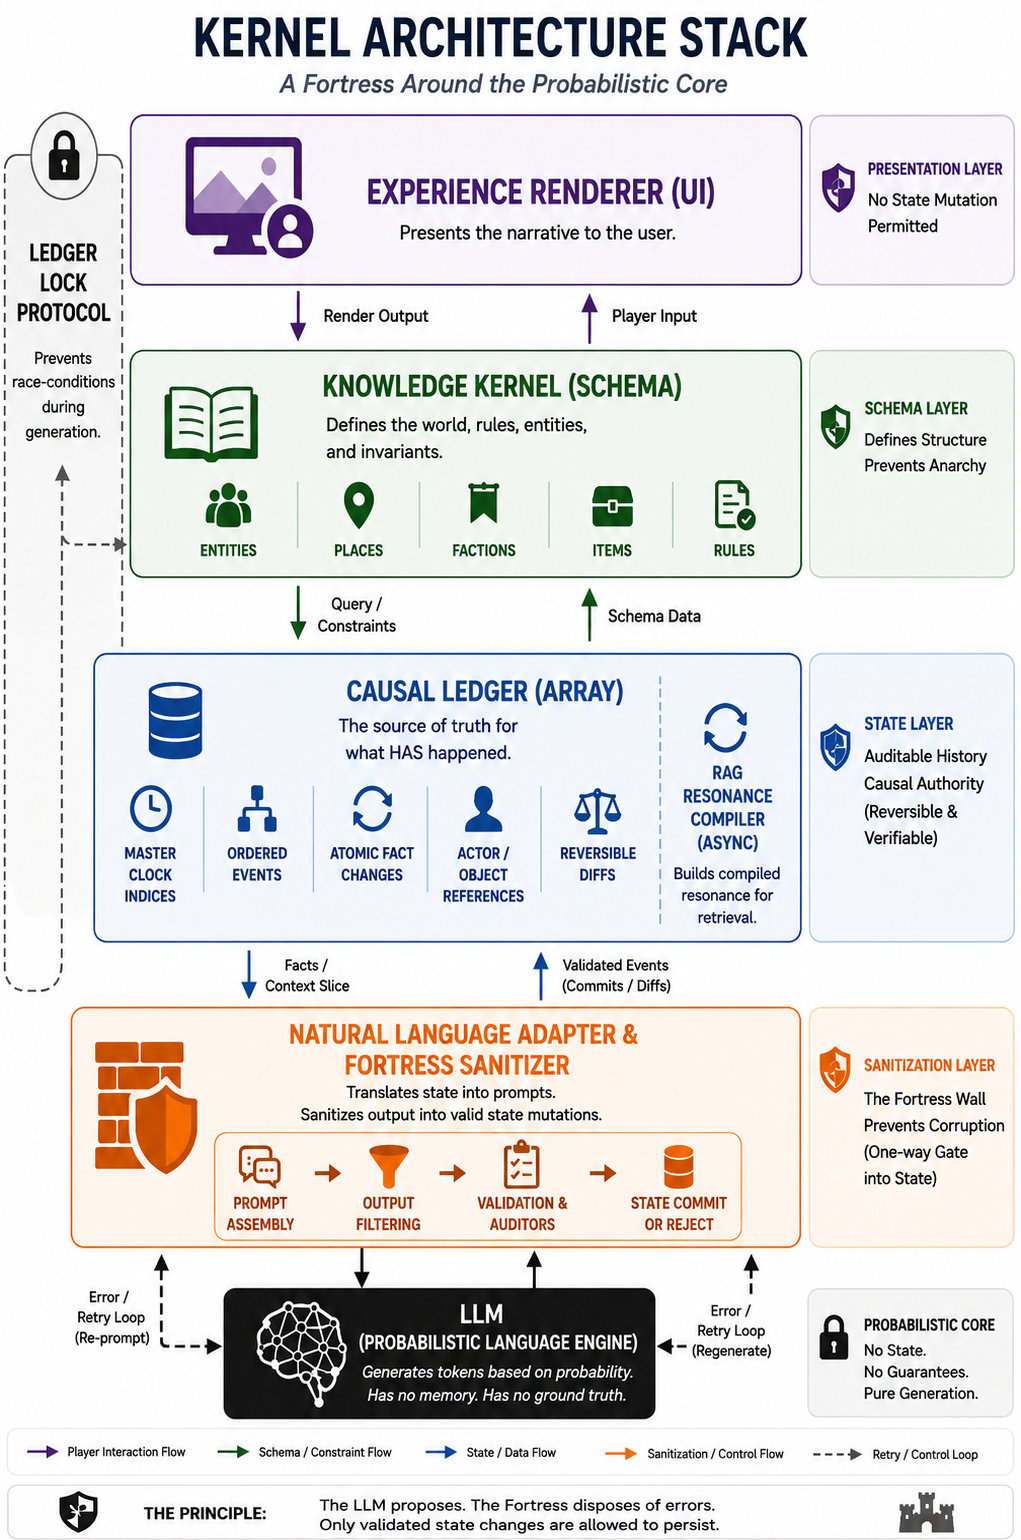
\includegraphics[width=\textwidth, height=0.95\textheight, keepaspectratio]{images/fig_kernel.png}
    \caption{The KERNEL stack. The probabilistic LLM is strictly subordinated. The Narration Adapter isolates the generative layer, while the Fortress Sanitizer ensures that only structurally valid, schema-compliant JSON is committed to the Causal Ledger.}
    \label{fig:kernel}
\end{figure}

\subsection{Component I: The Narrative Kernel}
\label{subsec:kernel}

The Narrative Kernel is the \textit{contract} your Narration Adapter must honor. It is the initial state matrix of your world before Turn 1 even begins. 

In a state-anemic system, this is usually just a giant "System Prompt" text box. In TomeWeaver, the Kernel (\texttt{setup.json}) is a strict JSON schema containing world entities, narrative tone, mortality flags, inventory rules, and (in Campaign mode) the rigid plot outline. 

The engine uses this schema to assemble the prompt dynamically at runtime, injecting only the fragments necessary for the current turn. This modularity means the Kernel can be versioned, diffed, and shared. Treat breaking changes to your world lore the same way you would treat a database migration.

\subsection{Component II: The Causal Ledger}
\label{subsec:ledger}

Every turn generated by the engine is a structured record, not a string of text. The Causal Ledger (\texttt{history.json}) tracks the player's choice, the generated prose, the location string, an optional snapshot of the inventory (where tracking is enabled), and any terminal flags (like \texttt{is\_game\_over}).

Crucially, every record is bound to the \textbf{Master Clock}---a strict, relative temporal coordinate system assigned by the Python backend. LLMs are notoriously incapable of tracking absolute time or counting accurately over long contexts. By externalizing the temporal axis into the Master Clock, the engine guarantees that causality only flows in one direction, ensuring that every committed turn is structurally \textbf{immutable from the perspective of the AI} (the model is physically locked out of altering history, while the human Director retains full administrative editing rights).

There is a common misconception about ledgers: people assume they must be strictly append-only (immutable). In this architecture, that is false. We define "immutability" not as the restriction of human administrative edits (the Director possesses full sovereign rights to execute surgery), but as the complete lockout of the AI from modifying past states. Once a turn is committed, the stochastic Prose Engine can never alter it. The integrity of the ledger comes from ensuring that every mutation is an explicit, named operation that triggers a deterministic re-indexing of the Master Clock, rather than silently deleting lines in a text file.

\subsection{Component III: Fault-Tolerant Narrative Processing}
\label{subsec:prose}

I cannot stress this enough: The LLM is an untrusted, probabilistic black box. In the LSM architecture, the language model is demoted. It is treated as an \textbf{unsafe probabilistic coprocessor}. The Narration Adapter is the deterministic CPU built to contain it. The Adapter's job is to assemble the context, request a structured JSON payload from the API, and aggressively validate the response before allowing it to touch the Causal Ledger.

The Sanitizer expects failure. It looks for rogue dialogue quotes breaking the JSON structure, patches missing array delimiters using error coordinates, and attempts regex recovery if the generation truncates mid-bracket. If all mechanical repairs fail, the engine translates the specific syntax error into a feedback prompt and forces the LLM to try again.

\subsubsection{Bounded Stochasticity}
In a state-rigorous system, hallucination is downgraded from a fatal system error to \textbf{Safeguarded Divergence}. This shift contributes to \textbf{Hardware Democratization} by reducing dependence on frontier-scale models. While these large scale models (400+ Billion parameters) exhibit high inherent reliability, TomeWeaver is optimized for consumer-grade hardware. The LSM framework allows smaller, locally-hosted models (typically with 12 Billion parameters or fewer), which are naturally more prone to structural syntax errors, to function as dependable engines. 

In a standard chat UI, developers are often forced to drop the model's temperature to near zero to ensure "safety," which results in repetitive, sterile prose. In an LSM architecture, we achieve \textbf{Bounded Stochasticity} by separating the pipeline's temperature parameters: while internal evaluation passes (RAG summarization and campaign auditing) are locked to a deterministic 0.1, the creative prose pass operates at a standard 0.8. Crucially, the Director is granted manual control over this generative envelope during "Fix" operations, scaling the model's creative freedom from a strict 0.1 to a highly divergent 0.9. Even if a high-temperature generation fails, the structural boundaries of the Fortress ensure the ledger remains uncorrupted.


\subsection{Component IV: The Experience Renderer}
\label{subsec:render}

The renderer is entirely replaceable. TomeWeaver ships with a Python/CustomTkinter desktop UI featuring a single-card timeline visualization, a Memory \& Lore console, and Markdown/HTML exporters. However, because the core logic is entirely decoupled from the GUI, the exact same engine could be wrapped in a CLI, deployed behind a Flask web API, or hooked into a Unity game engine tomorrow. The Experience Renderer simply translates the math of the ledger into human interface.


\vspace{0.5em}
\begin{figure}[htbp]
    \centering
    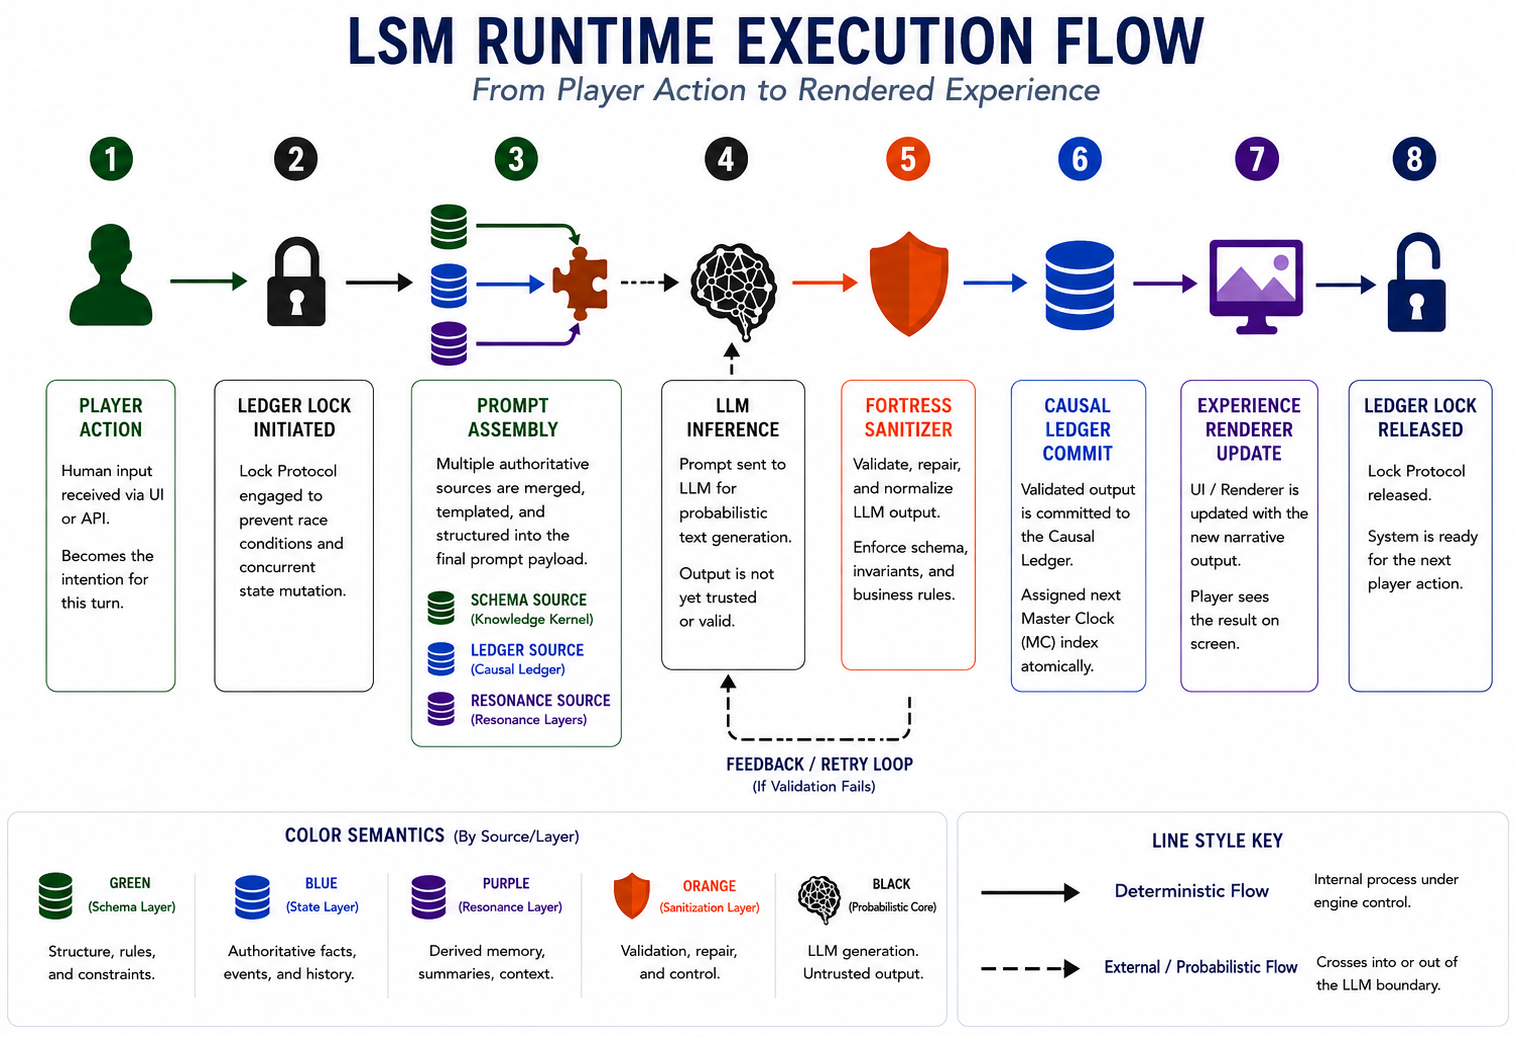
\includegraphics[width=\textwidth]{images/fig_execution.png}
    \caption{The LSM Runtime Choreography. This sequence illustrates the lifecycle of a single turn. Notice that the state machine is locked prior to prompt assembly, and the generated payload must survive the sanitization and audit gates before it is committed to the Causal Ledger.}
    \label{fig:execution}
\end{figure}



\newpage
% -------------------
% Section 5 - Ontological Resonance Layers and Substrate Scoping
% -------------------
\section{Ontological Resonance Layers and Substrate Scoping}
\label{sec:memory}

\subsection{The Illusion of Infinite Context}

When discussing long-term memory in AI, the immediate objection is usually hardware-based: \textit{Why build a complex Retrieval-Augmented Generation (RAG) system when models like Gemini or Claude offer context windows of over a million tokens? Why not just stuff the entire history into the prompt and let the model figure it out?}

Because capacity is not the same as comprehension. 

Even when a model \textit{can} hold a hundred thousand words in memory, feeding it that much raw data on every single turn introduces massive API latency, exorbitant token costs, and---for local users---a VRAM requirement that prices out 90\% of consumer hardware. More importantly, massive prompts suffer from attention dilution. Facts buried in the middle of a 500-turn transcript get ignored just as often as facts missing entirely. 

The LSM pattern is not just about remembering; it is about computational efficiency. Extending the principles of Retrieval-Augmented Generation \citep{lewis2020rag}, we compress raw history into \textbf{Ontological Resonance Layers}---dense, queryable memory fragments injected at prompt-build time---while the raw turns remain untouched on disk for human auditing.

\textit{Scope Honesty:} In the context of this implementation, Retrieval-Augmented Generation (RAG) refers to targeted, deterministic retrieval from structured JSON ledgers rather than vector-similarity search. By using explicit aliases, exact-match scoping, and chronological chunking, the engine guarantees that narrative facts are reliably injected without the stochastic failure rates inherent to calculating embedding distances.

\subsection{The Dual-Ledger Architecture}

TomeWeaver achieves this compression by running two distinct memory ledgers in parallel:

\begin{enumerate}
    \item \textbf{The Plot Ledger (Chronological Memory):} During standard play, the Experience Renderer automatically monitors milestones on turn resolution, calling the Resonance Compiler in a background thread to silently chunk past turns (typically using the default \texttt{context\_window} size of 10 turns) and asking the LLM to summarize the narrative arc. When a chapter concludes, these Part Summaries are further condensed into a high-level Chapter Summary. This tiered compression preserves the overarching plot while slashing token costs by orders of magnitude.
    \item \textbf{The Entity Ledger (Stateful Memory):} This is an object-oriented memory bank tracking Characters, Locations, Artifacts, and Factions. During compilation, the engine extracts new traits and chronological events, appending them to specific entity profiles. Entities are not continually re-invented by the LLM; they are retrieved from the database.
\end{enumerate}

To prevent the prompt from bloating with irrelevant data, an \textbf{Auto-Decay} algorithm monitors the timeline. If an entity is not mentioned in the prose or location tags for forty turns, it is automatically downgraded from "Active" to "Archived" and removed from the prompt injection. If the user or the AI mentions their name again, they instantly revive. It is a highly efficient attention model mimicking human recall.

\subsection{Substrate Scoping and Shared Universes}

The true power of separating state from prose becomes apparent when you scale beyond a single story. TomeWeaver introduces \textbf{Shared Universes}---multi-threaded multiverses where parallel stories inherit data from a single Global World Bible.

Managing memory across multiple threads introduces the risk of cross-contamination. We solve this through \textbf{Substrate Scoping}, which governs how the Narration Adapter injects memory:

\begin{itemize}
    \item \textbf{Local Scope:} The entity exists only in the current thread's \texttt{memory.json} (e.g., a minor tavern owner, a thread-specific plot twist).
    \item \textbf{Global Scope:} The entity lives in the universe's \texttt{shared\_memory.json}. All authorized threads merge this global lore into their prompts automatically.
    \item \textbf{Local Override (Prequel Shadowing):} If the same entity name exists in both the Global and Local ledgers, the engine prioritizes the Local data. This allows a user to play a flashback thread where the "Benevolent King" profile shadows the present-day "Tyrant King" profile, without destructively overwriting the global canon. 
\end{itemize}

\textbf{A Note on Synchronization:} Cross-thread consistency in TomeWeaver is file-based and resolved at prompt-assembly time; it is not a live multiplayer sync protocol. If Thread A burns down the Global Space Station, Thread B observes the ashes \textit{only after} Thread A's updates persist to disk and Thread B assembles its next prompt. 



\subsection{Continuity Auditing and Pre-Commit Validation}

Because LLMs hallucinate, the Resonance Compiler will inevitably make mistakes when summarizing history. TomeWeaver treats this as a QA problem. 

The engine provides a suite of retroactive auditing tools. The user can run a Fidelity Check, forcing the LLM to compare its own generated summary against the raw history turns and assign itself an accuracy score. If the report highlights contradictions, the Director can click "Auto-Patch," instructing the AI to rewrite the summary using the QA report as a strict guideline. 

Visualizing these overlapping ontological layers requires a clear understanding of the substrate hierarchy. In a multi-threaded multiverse, the state machine acts as a prism, refracting global truths through the specific lens of a local thread. This ensures that the Narration Adapter reconciles diverging histories without compromising the integrity of the primary world bible. By explicitly defining these shadowing barriers, the engine guarantees that causality remains consistent within each specific narrative substrate while allowing for the emergence of non-linear parallel play.

\vspace{1em}

\begin{figure}[hbt!]
    \centering
    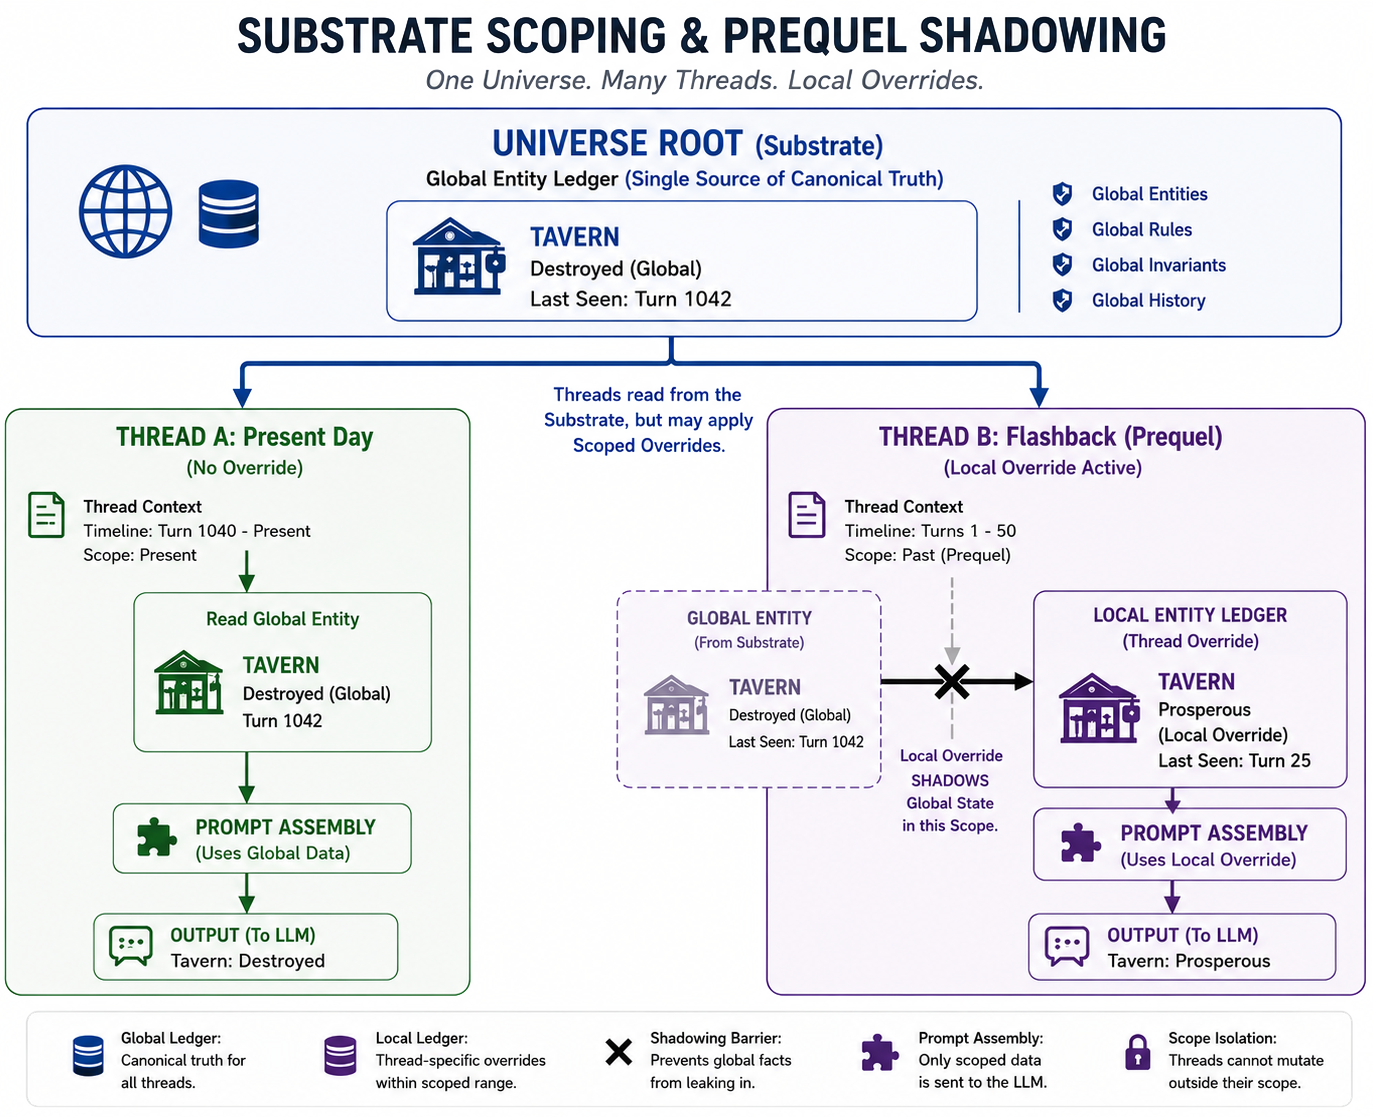
\includegraphics[width=1\textwidth]{images/fig_substrate.png}
    \caption{Substrate Scoping and Prequel Shadowing. The Shared Universe holds Global entities (top). Thread B utilizes a Local Override to shadow the Global canon without destructively overwriting it. The Prompt Assembly strictly injects the correct substrate per thread.}
    \label{fig:substrate}
\end{figure}

This rigorous auditing extends proactively to external data. When a Director attempts to bulk-import unstructured prose into the timeline, the engine uses the RAG system as an advisory \textbf{Pre-Commit Gatekeeper}. It scores the foreign text against the active Local and Global entity ledgers, flagging continuity violations, tonal shifts, or character mismatches to provide the Director with an integration report before they authorize the splice.

In a state-rigorous system, memory is not trusted; it is verified.


\newpage
% -------------------
% Section 6 - Causal Revisionism: Timeline Surgery
% -------------------
\section{Causal Revisionism: Timeline Surgery}
\label{sec:surgery}

\subsection{The Editor's Problem}

If you run a campaign long enough, you will eventually need to perform structural surgery on the narrative. You will need to delete a dead-end turn, insert a forgotten conversation, split a sprawling chapter in two, or fork a compelling side-quest into its own dedicated story thread. 

In a transcript-centric chat UI, these operations are manual nightmares. You are forced to copy-paste blocks of text into external editors, lose your place in the narrative, and pray the LLM understands the new context when you paste it back. 

In TomeWeaver, editorial intervention is not a hack; it is a first-class state transition. We designate these operations collectively as \textbf{Causal Revisionism}.

\subsection{The Algebra of Editing}

Drawing upon the database principles of Event Sourcing \citep{fowler2005} and Command Query Responsibility Segregation (CQRS) \citep{young2010cqrs}, TomeWeaver models narrative state as a sequence of discrete events. Because the Causal Ledger is an indexed array of JSON objects rather than a flat string, operations that would shatter a plain-text transcript are reduced to basic array mathematics. The engine supports a robust edit algebra:

\begin{description}
    \item[Insertion:] The Director inserts a blank turn card between Turn 14 and Turn 15. The Master Clock mechanically right-shifts all subsequent turns (+1) and updates the bounding integers in \texttt{chapters.json}.
    \item[Deletion:] A turn is removed. Downstream indices left-shift (-1), and the \texttt{player\_choice} causality is migrated to the preceding turn so the narrative chain does not break.
    \item[Bridge Conversion:] A raw player action is collapsed forward, stored as \texttt{narrative\_bridge} metadata on the next card, preserving the curated scene prose while maintaining the flow of time.
    \item[Chapter Splicing:] The Director selects Chapters 1 and 3. The engine extracts those specific turns, generates a new \texttt{history.json}, \textbf{deterministically} re-indexes the master clock to close the gap, and clones the setup schema to spawn a perfect, standalone cartridge.
    \item[Bulk Import:] External prose (from MS Word or another AI) is pasted in. The engine parses action markers (e.g., \texttt{>}), chunks the text into valid JSON turn cards, and splices the massive block directly into the timeline.
\end{description}

Each of these operations preserves the principle of Non-Destructive Orchestration. The Director remains in absolute control: mechanical timeline surgery (such as inserts or deletions) is validated via explicit confirmation dialogues, while AI-proposed draft mutations (such as expansions or fixes) are highlighted in the Red/Green visual diff viewer before committing. The Prose Engine is completely blind to timeline surgery; it simply receives the cleanly compiled, post-surgery state on the next API call.

\subsection{Counterfactual Versioning}

In a transcript-centric interface, exploring a "What If?" scenario is destructive. You either overwrite your current state, or you branch blindly into a new window, losing all metadata and RAG context in the process. 

TomeWeaver elevates the Causal Ledger from a single linear array into a \textbf{Directed Acyclic Graph (DAG)} of narrative states. We expose this via the Run Tree. The engine manages parallel timelines at the file-system level using discrete snapshots and a central routing manifest. 

A Director can fork a timeline at Turn 15, play out a disastrous combat encounter, save the branch, and instantly swap the root state back to the original Turn 15 to explore the diplomatic approach. Because the state swap is handled physically at the file-system root, there is zero context-bleed between the branches. It is essentially Git for interactive fiction: the non-destructive exploration of parallel realities without ever corrupting the root canon.

\subsection{The Ledger Lock Protocol}
\label{subsec:lock}

When you decouple the user interface from the generation loop, you introduce the risk of \textbf{Ontological Race Conditions}. 

Imagine the Prose Engine is currently running on a background thread, writing a dramatic death scene for a character at Turn 11. Meanwhile, the impatient user navigates back to Turn 10 in the UI and clicks "Delete Character." If the system processes that user input, reality forks mid-commit. The LLM returns a payload referencing an entity that no longer exists in the state machine, causing a catastrophic data collision.

To prevent this, TomeWeaver implements the \textbf{Ledger Lock Protocol}. While the Narration Adapter is actively awaiting a response from the LLM during the provisional generation phase, the engine engages the Ledger Lock, disabling all timeline navigation and inline surgery triggers to protect the generative hot-path. However, once the provisional turn is rendered and the lock is released, any subsequent memory compilation runs asynchronously as a non-blocking background thread. Because this compiler writes to separate, isolated state ledgers, the Director remains free to explore, edit, or traverse the timeline without waiting for the compilation to finish.

The lock is not elegant theoretical computer science; it is the blunt, necessary difference between an engine you can trust and one that silently corrupts its own causal graph.

\textit{Scope Honesty:} The reference lock in TomeWeaver is UI-level and designed for single-session local play. If you were to adapt the LSM architecture for a server-side application with multiple concurrent users, Layer L would need to be upgraded with strict database transactions or optimistic concurrency tokens.


\newpage
% -------------------
% Section 7 - The Director Role: Ontological Agent and Epistemic Agency
% -------------------
\section{The Director Role: Ontological Agent and Epistemic Agency}
\label{sec:agent}

\subsection{Asymmetric Co-Creation}

In the Chatbot Era, the user is a \textit{Prompter}. Their primary verb is negotiation. They type a request into a box, cross their fingers, and beg the model to honor the constraints of the world. 

The Language State Machine transforms the operator into a \textbf{Director}. In TomeWeaver, the Director does not negotiate with the language model; they govern the state machine. They author the Narrative Kernel, trigger memory compilations, authorize timeline surgery, accept or reject visual diffs, and set the scoping rules for shared universes.

This shift in control topology is what I call \textbf{Asymmetric Co-Creation}. You and the AI are not equal co-authors. The human owns the state; the machine owns the syntax. The Director commits absolute facts to the ontological ledger, and the Prose Engine is merely permitted to propose candidate prose subject to validation, review, and lock discipline. 

\subsection{Epistemic Agency}

Because the system state is externalized into queryable ledgers rather than buried in a transcript, the pleasure of interacting with the software fundamentally changes. 

In a traditional choose-your-own-adventure game, player agency is expressed through branching paths (choosing Door A or Door B). In TomeWeaver, the most powerful actions often have nothing to do with advancing the plot. A Director might spend an hour \textit{navigating state}---scrubbing the timeline to see how a decision on Turn 5 cascaded into a crisis on Turn 50, auditing the Entity Ledger for contradictions, pinning a villain's profile so they never decay from the AI's active memory, or tracing the exact turn an artifact was added to the inventory.

We define the user in this capacity as an \textbf{Ontological Agent}. Their leverage is \textbf{Epistemic Agency}---power derived from understanding, managing, and forensically navigating the rules and records of the system. The story is not told \textit{to} the Agent; it is \textit{extracted} from the database. 

\subsection{Sandbox vs. Campaign Constraints}

The LSM architecture supports different levels of generative constraint, which TomeWeaver exposes as two distinct game modes:

\begin{itemize}
    \item \textbf{Sandbox Mode:} Designed for emergent, open-ended simulation. The Director exercises maximum sovereignty, manually forcing scene shifts, time jumps, and POV changes. The Prose Engine is constrained only by the static world lore and the active memory ledgers.
    \item \textbf{Campaign Mode:} Designed for guided, plot-driven narratives. The Narration Adapter is tightly bound to a pre-defined Plot Outline. The engine utilizes a hidden "Auditor" pass---a secondary LLM call acting as a strict semantic classifier. The Auditor reads the recent prose against the active micro-objective, returning a structured JSON evaluation. While individual turns continue to commit prose and player choices, the engine strictly forbids chapter progression and locks the next objective until the Auditor verifies that the goal has been achieved, preventing the model from hallucinating unearned victories.
\end{itemize}

Both modes share the exact same cartridge discipline, the same RAG compilation, and the same timeline surgery protocols. They differ only in which fields of the Narrative Kernel are allowed to bind the LLM during prompt assembly.

\subsection{The Director as the Ultimate Arbiter}

A fundamental constraint of generative simulation is the gap between \textit{structural validity} and \textit{narrative resonance}. While the Fortress Sanitizer (Section 4.3) can mathematically guarantee that an LLM’s output is a well-formed JSON object, it cannot verify if that output is actually \textit{good}. It can confirm that a "Choices" array contains a series of strings, but it cannot judge if those choices offer the player meaningful agency or if they are narratively non-sequiturs.

In the LSM framework, we acknowledge that while the machine is the master of syntax, the human Director is the \textbf{Sole Judge of Meaning}. The Director functions as a "Human-in-the-loop" governor who prevents the simulation from collapsing into a valley of technically valid but irrelevant prose. This role is not merely as a passive reader, but as a judicial authority over the Causal Ledger. Every turn proposed by the Prose Engine is treated as a \textit{candidate state} until the Director authorizes the commit.

This judicial authority is exercised through a specialized set of orchestration verbs that allow the Director to sculpt the narrative without advancing the Master Clock:
\begin{itemize}
    \item \textbf{Reroll:} A total rejection of the candidate turn. The Director determines the prose is irrelevant, out-of-character, or hallucinated, forcing the coprocessor to generate a fresh probability set.
    \item \textbf{Expand/Condense:} Directives for pacing control. The Director acts as a developmental editor, requesting more sensory depth or a swifter narrative rhythm based on the intended emotional arc of the scene.
    \item \textbf{Polish:} A linguistic refinement pass. The Director corrects mechanical errors---typos, tense inconsistencies, or clunky phrasing---that the LLM might have introduced, ensuring the exported storybook maintains professional literary standards.
\end{itemize}

One might argue that these judgements could be off-loaded to a secondary layer of "Auditor" LLMs. However, the LSM architecture rejects this as a viable solo solution due to the \textbf{Economic Paradox of Orchestration}. Each additional layer of AI verification adds superlinear increases to token costs, API latency, and "Context Bleed," while offering diminishing returns in creative judgement. The human Director remains the most computationally efficient and narratively accurate tool for assessing the "soul" of a story. The Fortress was built to catch badly formed data; the human was kept in the loop to catch badly formed meaning.

\subsection{Ontological Stewardship and Operational Ethics}

The transition from "Prompter" to "Director" introduces a new form of creative responsibility which we term \textbf{Ontological Stewardship}. In state-anemic systems, narrative is disposable; if a story contradicts itself, the user simply abandons the session and starts a new one. The LSM architecture, by contrast, creates durable realities. Because the Causal Ledger is persistent and the Entity Ledger is cumulative, the Director’s choices have long-term "gravity." 

This durability necessitates an operational ethic. Stewardship requires the Director to maintain the \textit{Internal Veracity} of the simulation, even when the coprocessor offers "easy" or "convenient" hallucinations that advance the plot but break the world's logic. If the Director accepts a turn where a character magically recovers from a fatal wound without a mechanical reason, they are committing \textbf{Ontological Pollution} to the ledger. This pollution will eventually degrade the RAG Resonance Layers, leading to a cascade of further hallucinations.

The LSM architecture provides the tools for this stewardship, but it cannot enforce it. The "Time Travel" slider and the Timeline Surgery tools (Section 6) are the Director’s primary instruments for forensic cleanup. Curation is an act of maintenance. By treating the story as a database, the framework encourages a shift in user behavior: moving away from the "disposable output" culture of standard AI chat and toward a culture of "durable world-building." The Director is not merely telling a story; they are maintaining the health of a structured reality.

Ultimately, the goal of the Ontological Agent is to achieve \textbf{Narrative Synthesis}---the point where the stochastic brilliance of the LLM and the deterministic rigor of the ledger are so perfectly balanced that the simulation feels both emergent and inevitable. This synthesis is the highest state of the Language State Machine. It represents the successful transition from probabilistic noise to meaningful, persistent experience.


\newpage
% -------------------
% Section 8 - Implementing and Extending the Architecture
% -------------------
\section{Implementing and Extending the Architecture}
\label{sec:implement}

To bridge the gap between theoretical architecture and working software, Table \ref{tab:implementation} maps the abstract LSM concepts directly to their concrete implementations in the TomeWeaver codebase (at the time of this publication). 

\begin{table}[hbt!]
\centering
\caption{The Implementation Reality}
\label{tab:implementation}
\renewcommand{\arraystretch}{1.4}
\begin{tabular}{p{0.35\textwidth} p{0.55\textwidth}}
\toprule
\textbf{LSM Concept} & \textbf{TomeWeaver Implementation} \\
\midrule
Narrative Kernel & \texttt{setup.json} \\
Causal Ledger & \texttt{history.json} \\
Resonance Layers & \texttt{memory.json} (Summaries and entity ledgers) \\
Lock Protocol & UI-level local generation lock \\
Prompt Assembly & Externalized prompt fragments \\
Fortress Sanitizer & JSON repair and retry pipeline \\
Counterfactual Branching & File-system snapshots and the Run Tree manifest \\
\bottomrule
\end{tabular}
\end{table}

\subsection{Cartridge Conventions and Federated Exchange}

To ensure portability and version control, TomeWeaver serializes the entire state machine into a standardized directory structure we call a \textit{Cartridge}. A minimal story cartridge on disk looks like this:

\begin{verbatim}
adventures/MyStory/
  setup.json       # Narrative Kernel (Schema and Rules)
  history.json     # Causal Ledger (Indexed Turns)
  chapters.json    # Chapter Topology and Goal Tracking
  memory.json      # Compiled Ontological Resonance Layers (RAG)
\end{verbatim}

If the story is part of a Shared Universe, the engine dynamically traverses up the directory tree to merge data from a parent \texttt{master\_setup.json} and \texttt{shared\_memory.json}. 

That is the entire physical contract. There are no obfuscated databases or proprietary binary blobs. You can inspect it, back it up to a flash drive, diff it in Git, or share it as a ZIP file.

This modularity enables \textbf{Federated Timeline Exchange}. Because the state is decoupled from the engine, users can export differential "Branch Packs"---snapshots containing only their diverging timeline ledgers without the root schema. 

To prevent catastrophic data collisions when merging a foreign timeline into a local cartridge, the engine performs \textbf{Ontological Checksumming}. It hashes the Narrative Kernel (the world rules, tone, and campaign outline) to create a deterministic fingerprint. It acts as an advisory warning system, alerting the Director of any ontological mismatches while preserving their ultimate sovereignty to override the warning and force the merge. A user is thus protected from accidentally splicing a hard-sci-fi timeline into a high-fantasy RAG database, while retaining the freedom to do so intentionally.

\subsection{Extension Points}

TomeWeaver is a reference implementation, not a walled garden. Developers building upon the LSM architecture are encouraged to swap or extend the KERNEL layers:

\begin{itemize}
    \item \textbf{Resonance Compiler:} Replace the LLM summarization pass with deterministic rules, vector embeddings, or hybrid retrieval systems.
    \item \textbf{Narration Adapter:} Swap local API endpoints for cloud providers, or implement specialized schema validators tailored to specific game genres (e.g., a hard-sci-fi ruleset).
    \item \textbf{Renderer:} Discard the CustomTkinter desktop UI entirely. Wrap the core Python engine in a CLI, a web framework, or a plugin for a 3D game engine.
    \item \textbf{Lock Layer:} Upgrade the single-tenant UI lock to support distributed database transactions for multi-user, server-side deployments.
\end{itemize}


\subsection{Headless Validation and the Simulation Sandbox}

A critical requirement for any production-grade narrative engine is the ability to validate system logic without a human interface. TomeWeaver achieves this through a strictly \textbf{Headless Core}. The engine logic resides entirely within the \texttt{BaseEngine} class and its derivatives, which communicate via standard Python dictionaries. This decoupling allows for the execution of the \texttt{Run\_Tests.bat} suite, a collection of more than 250 automated tests that mathematically prove the integrity of the Master Clock, the safety of timeline surgery, the precision of the JSON "Fortress" Sanitizer, and various other parts of the software (unit testing).

Furthermore, the framework supports \textbf{Closed-Loop Convergence Testing} (Autopilot) via the presentation layer. The Director can trigger an automated, closed-loop traversal of the active timeline, forcing the engine to automatically select the primary choice on every turn. This serves as an automated, exploratory stress-test: allowing the Director to observe how the campaign’s chapter exit-nodes and final victory/termination states respond to repeated turn transitions over long sessions. By treating the campaign as an empirically testable software object, the LSM framework moves generative narrative out of the realm of "prompt-guessing" and into the realm of verifiable systems engineering. These backend patterns are designed to be portable to any environment---from web servers to 3D game engines---without requiring the porting of the CustomTkinter graphical interface.


\newpage
% -------------------
% Section 9 - Proposed Evaluation Metrics
% -------------------
\section{Proposed Evaluation Metrics}
\label{sec:falsifiability}

We state the following as \textbf{research hypotheses} for comparative study. They are explicitly framed as falsifiable metrics for anyone who wishes to benchmark LSM sessions against standard transcript baselines.

\begin{description}
    \item[H1: Continuity Half-Life.] Define a contradiction rate (via manual audit or automated entity cross-checking) plotted against turn count. \textit{Hypothesis:} State-anemic baselines will exhibit a contradiction rate that grows superlinearly as the context window fills. LSM sessions with active RAG compilation will exhibit a bounded, stable contradiction rate over the same turn count, holding the base model and token budget constant.

    \item[H2: Recovery Cost.] Measure the time (or number of edit operations) required for a human operator to fix an injected continuity error. \textit{Hypothesis:} Explicit timeline surgery and visual diffs require significantly less recovery time than regenerate-and-scroll workflows in chat interfaces.

    \item[H3: Cross-Thread Consistency.] In a shared-universe setup, Thread A writes a Global entity update to \texttt{shared\_memory.json}. \textit{Hypothesis:} Thread B's subsequent prompt assembly will reliably reflect that update without requiring manual copy-paste intervention, verifiable by diffing the injected memory payloads.

    \item[H4: Audit Value.] \textit{Hypothesis:} At a fixed prompt token budget, injecting fidelity-scored RAG summaries reduces contradiction rates in generated prose compared to injecting truncated raw history. Measurable via blind continuity reviews.
\end{description}

TomeWeaver's verbose logging hooks (\texttt{log\_verbose}, raw JSON failure traces) and headless test suites exist precisely to support such benchmarks. While current LLM leaderboards (such as MMLU or GSM8K) measure static reasoning or coding proficiency, they fail to account for the \textbf{Temporal Resilience} required for persistent simulation. Our proposed metrics move beyond the "one-shot" response, challenging models to maintain a coherent reality across a multi-turn causal graph. 

By standardizing these evaluations, the community can begin to rank models not just on their linguistic flair, but on their \textit{Ontological Obedience}---their ability to respect a Narrative Kernel and a Causal Ledger without introducing amnesia-driven contradictions. We believe that this shift toward state-rigorous benchmarking is a necessary prerequisite for the development of truly autonomous, persistent AI worlds. Running these evaluations at scale remains a primary objective for the Meaningfulness Media Group and the broader open-source community.



\newpage
% -------------------
% Section 10 - Discussion
% -------------------
\section{Discussion}
\label{sec:discussion}

\subsection{Separation of Concerns}

The AI industry keeps asking: \textit{How do we prompt the model to remember better?} 

The LSM pattern asks a ruder question: \textit{Why should the model be the memory at all?} 

Declarative rules belong in the Kernel. Committed events belong in the Ledger. Compressed recall belongs in the Resonance Compiler. The LLM simply proposes candidate wording; the wrapper decides what becomes canon. That separation of concerns sounds like boring, boilerplate computer science---until you have spent a week trying to debug a 300-turn RPG campaign that violated it. 

\subsection{Axiomatic Investment and Compounding Returns}

State-anemic tools offer zero-interest storytelling. They are effortless to start, but their narrative value rarely compounds. Each session begins from a thin transcript, and Turn 200 pays roughly the same amnesia tax as Turn 20. 

The LSM pattern demands \textbf{Axiomatic Investment}---the upfront, sometimes tedious labor of defining schemas, scopes, ledgers, and compilation policies. But it yields \textbf{Compounding Narrative Returns}. Every turn played enriches the Ontological Resonance Layers. Entity histories deepen. Plot summaries stack. Universe substrates accumulate canon. Turn 500 can be richer, more historically accurate, and more texturally dense than Turn 1, not despite the machinery, but because of it. 

Short improvisational sessions may not amortize that setup cost; a multi-chapter campaign or a shared world usually will.

\subsection{Relation to Prior Work}

The Language State Machine sits at the intersection of classical hyper-narrative theory and modern probabilistic inference. Our architectural goals align closely with the four essential properties of digital environments defined by \citet{murray1997}: they must be \textit{procedural}, \textit{participatory}, \textit{spatial}, and \textit{encyclopedic}. 

Standard state-anemic chatbots often fail Murray's "procedural" requirement; while they generate text, they lack the underlying engine rules to resolve a player's action with consistency. By externalizing state into the Narrative Kernel and Causal Ledger, we provide the procedural scaffolding necessary for a "Cyberbard" to function reliably. Furthermore, our tiered RAG architecture (Section 5) fulfills the "encyclopedic" property, allowing the narrative to draw upon a deep, structured repository of world lore that exceeds the capacity of a simple chat transcript.

This framework also builds upon historic experiments like \textit{Façade} \citep{mateas2003}, which introduced narrative state machines but relied on hand-authored dialogue "beats" rather than Large Language Models. While the concept of an AI "Drama Manager" is well documented \citep{weydhraad2001}, earlier implementations usually relied on rigid Finite State Machines \citep{buckland2001}. The LSM architecture modernizes these concepts, replacing hardcoded transitions with \textbf{Safeguarded Divergence} (Section 4.3.1), allowing for the emergent creativity of contemporary agents \citep{park2023agents} without sacrificing the structural discipline required for long-form continuity. This technical rigor serves not merely as an engineering safeguard, but as the prerequisite for a broader shift in our conceptual understanding of what it means to build and sustain a digital reality.


\subsection{The Evolution of Speculative Modeling}

The Language State Machine represents a significant shift in the management of generative narrative; it moves beyond the linear storytelling traditions that have largely governed digital expression. Recent advances in generative systems now provide a substrate capable of unprecedented improvisational flair. However, as we have argued, flair without structural discipline is insufficient for sustained simulation. 

The LSM framework, alongside its macro-sociological sibling, the \textbf{Speculative Ontological Engine (SOE)} \citep{bee2025soe}, establishes a methodology we term \textbf{Generative Realism}. Both frameworks operate on a shared philosophical axiom: \textit{reality is a ledger}, and narrative is a subjective rendering of that ledger's state. 

While the SOE operates at the macro-scale---modeling the trajectories of civilizations across centuries---the LSM operates at the micro-scale of the turn-by-turn experience. Together, they form a recursive hierarchy of stateful simulation. In this paradigm, the role of the human operator shifts from "Authoring Prose" to \textbf{Architecting Invariants}. The primary creative act is no longer the manual scripting of every interaction, but the definition of the physical, social, and ontological laws of the world, followed by the orchestration of the AI’s probabilistic exploration of that space.

\subsubsection{Architectural Portability: Beyond Narratology}

The implications of this state-rigorous architecture extend to any domain where persistent probabilistic systems require durable state governance. By treating the Large Language Model as a coprocessor within a deterministic framework, the LSM pattern can be applied to complex modeling scenarios outside of interactive fiction:
\begin{itemize}
    \item \textbf{Jurisprudence and Policy:} Utilizing the "Causal Ledger" to track the long-term, cascading effects of variable policy changes within a persistent simulation of a legal environment.
    \item \textbf{Counterfactual Research:} Reconciling divergent causal branches in historical or strategic modeling by modifying the "Narrative Kernel" and auditing the system's response.
    \item \textbf{Organizational Dynamics:} Maintaining "invariant constraints" (resources, logistical limits, morale) in high-stakes training simulations where the AI manages the dialogue but the engine enforces the reality.
\end{itemize}

We are entering a phase where the distinction between "Fiction" and "Simulation" becomes increasingly porous. The LSM provides the skeletal integrity required for these virtual realities to maintain coherence over long durations. Whether the objective is literary or analytical, the requirement for \textbf{Ontological Stewardship} remains constant: the machine must be caged by state, and the human must remain the final arbiter of meaning.


\subsection{Limitations (Explicit)}

To be clear about what this architecture does \textit{not} solve:

\begin{itemize}
    \item \textbf{Lossy Summarization:} RAG compression is inherently lossy. While major causal events are preserved, subtle subtext or minor environmental clues in the raw history may be discarded during condensation if not explicitly extracted into the Entity Ledger.

    \item \textbf{Generative Ceiling:} Narrative quality remains bound by the capabilities of the underlying model. A state-rigorous architecture prevents amnesia but cannot force a low-parameter model to write at a professional literary level.

    \item \textbf{Director Cognitive Load:} The role of the Ontological Agent requires significant active engagement. The shift from passive consumer to active system steward may, for some users, represent an unwelcome increase in cognitive labor.

    \item \textbf{Synchronization Scoping:} Universe-level consistency is managed via a file-based protocol. It is not a distributed multiplayer engine and does not currently support real-time concurrent state mutation across different machines.

    \item \textbf{Transaction Integrity:} UI-level locks prevent local race conditions during single-user play, but the framework lacks the row-level locking or ACID-compliant transactions required for enterprise-scale multi-user environments.
\end{itemize}

Furthermore, the TomeWeaver reference implementation is licensed under Polyform Noncommercial 1.0.0. The architectural patterns described in this paper, however, are offered under CC BY 4.0 for share, reuse, critique, and adaptation.



\newpage
% -------------------
% Section 11 - Generalizing the Architecture: Beyond Interactive Fiction
% -------------------
\section{Generalizing the Architecture: Beyond Interactive Fiction}
\label{sec:generalize}

Throughout this paper, we have used the vocabulary of interactive fiction: stories, chapters, protagonists, and prose. However, interactive fiction is merely a proving ground. Text is simply the most computationally efficient substrate for stress-testing state-management logic. 

When the architecture is abstracted, it becomes clear that the Language State Machine is not limited to text adventures. It is a generalized architecture for persistent generative simulation systems.

\subsection{AI-Assisted Game State Orchestration}

If we swap the Experience Renderer from a desktop text UI to a 3D spatial engine like Unity or Unreal, the LSM pattern remains entirely intact. The Causal Ledger functions as the game's save file. The Ontological Resonance Layers allow non-player characters (NPCs) to possess computationally cheap, practically infinite memory of the player's past actions. The LLM is no longer generating a paragraph of text; it is generating a JSON payload containing dialogue arrays, animation triggers, and pathfinding coordinates, all validated by the Fortress Sanitizer before rendering.

\subsection{Persistent Multi-Agent Realities}
While systems like Generative Agents \citep{park2023agents} proved that autonomous NPCs can simulate complex societies, prompting dozens of agents simultaneously is too heavy and token-expensive for long-term consumer use. By applying the LSM's Substrate Scoping and Auto-Decay rules, a system could simulate a persistent town of hundreds of agents. The engine tracks their interactions deterministically in the background ledgers, only invoking the Prose Engine to render the exact dialogue or actions of the agents the human user is actively observing. 

\subsection{Procedural Lore Auditing}
In massive multiplayer games or tabletop franchises, lore often contradicts itself over years of expansions. An LSM could be deployed purely as a headless continuity auditor for human writers. Utilizing the Pre-Commit Validation pipeline (Section \ref{sec:memory}), new writing could be mechanically scored against established Global Entity ledgers, ensuring that new expansions do not violate the established World Bible.

By decoupling state from generation, the LSM pattern establishes a framework where AI is no longer treated as a volatile magic trick, but as a reliable, integrated component of complex systems engineering.




% -------------------
% Section 12 - Conclusion
% -------------------
\section{Conclusion}

The Language State Machine externalizes story state into inspectable layers: a schema kernel, a causal ledger, compiled memory, validated narration, and explicit operational locks. TomeWeaver demonstrates that this pattern is implementable today---on disk, headless, and testable---without waiting for a monolithic, multi-million token context window to save us from our own bad architecture. 

This document is meant as a buildable reference. Take the layers you need. Swap the renderer. Fork the compiler. Measure continuity if you are skeptical.

The era of the infinite scroll is reaching its structural limit. Whether you are building long-form interactive fiction, persistent multi-agent simulations, or enterprise data workflows, the lesson is the same: \textbf{you cannot rely on a probabilistic text-predictor to maintain absolute state.}

By externalizing world state and enforcing strict ledger discipline, generative simulation becomes a solvable systems engineering problem. The goal is no longer to chat with an AI. The goal is to architect a reality, treat the LLM as a sandboxed rendering engine, and orchestrate the transitions.

Play the simulation. Export the novel. Audit the ledger.






% -------------------
% About the Author
% -------------------
\vspace{1cm}
\section*{About the Author}

\textbf{Djeff Bee} is the Principal Architect at Meaningfulness Media Group and the creator of the \textit{Speculative Ontological Engine} (SOE) and \textit{TomeWeaver}.

Djeff Bee is the professional pseudonym of \textbf{Dominic Branchaud}, a senior research engineer with more than twenty-five years of experience in computer graphics, computer vision, and immersive simulation systems. His career has included roles at \textbf{CSIRO Data61}, \textbf{UNSW EPICentre}, and the \textbf{Laboratory of Research in Imaging for Orthopedics (LIO)}.

He has authored peer-reviewed publications (ACM SIGGRAPH, IEEE, SPIE) and holds multiple patents in 3D reconstruction and imaging. TomeWeaver applies simulation-style state management---structured data, non-destructive editing, and auditable pipelines---to long-form generative narrative.

\vspace{2em}





\newpage
% -------------------
% Bibliography
% -------------------
\bibliographystyle{plainnat}
\begin{thebibliography}{9}

\bibitem[Bee(2025)]{bee2025soe}
Bee, D. (2025). \textit{A Methodology for Generative Narrative and Civilization-Modeling: The Speculative Ontological Engine (SOE) Framework}. Meaningfulness Media Group.

\bibitem[Buckland(2001)]{buckland2001}
Buckland, M. (2001). \textit{Programming Game AI by Example}. Wordware Publishing, Inc.

\bibitem[Fowler(2005)]{fowler2005}
Fowler, M. (2005). \textit{Event Sourcing}. \url{https://martinfowler.com/eaaDev/EventSourcing.html}.

\bibitem[Lewis et al.(2020)]{lewis2020rag}
Lewis, P., Perez, E., Piktus, A., Petroni, F., Karpukhin, V., Goyal, N., Küttler, H., Lewis, M., Yih, W., Rocktäschel, H., Riedel, S., \& Kiela, D. (2020). Retrieval-Augmented Generation for Knowledge-Intensive NLP Tasks. \textit{Advances in Neural Information Processing Systems}, 33, 9459--9474.

\bibitem[Liu et al.(2023)]{liu2023lost}
Liu, N. F., Lin, K., Hewitt, J., Paranjape, A., Bevilacqua, M., Petroni, F., \& Liang, P. (2023). Lost in the Middle: How Language Models Use Long Contexts. \textit{Transactions of the Association for Computational Linguistics}, 12, 157--173.

\bibitem[Mateas and Stern(2003)]{mateas2003}
Mateas, M., \& Stern, A. (2003). Façade: An Experiment in Building a Fully-Realized Interactive Drama. \textit{Game Developers Conference (GDC)}, 2(3), 82--88.

\bibitem[Murray(1997)]{murray1997}
Murray, J. H. (1997). \textit{Hamlet on the Holodeck: The Future of Narrative in Cyberspace}. MIT Press.

\bibitem[Park et al.(2023)]{park2023agents}
Park, J. S., O'Brien, J. C., Cai, C. J., Morris, M. R., Liang, P., \& Bernstein, M. S. (2023). Generative Agents: Interactive Simulacra of Human Behavior. \textit{Proceedings of the 36th Annual ACM Symposium on User Interface Software and Technology (UIST '23)}.

\bibitem[Weyhrauch(1997)]{weydhraad2001}
Weyhrauch, P. (1997). \textit{Guiding Interactive Drama}. Ph.D. Dissertation, Carnegie Mellon University.

\bibitem[Young(2010)]{young2010cqrs}
Young, G. (2010). \textit{CQRS Documents}. \url{https://cqrs.files.wordpress.com/2010/11/cqrs_documents.pdf}.

\end{thebibliography}





\clearpage
% -------------------
% Appendices - Divider
% -------------------
\appendix

\thispagestyle{empty}
\vspace*{0.35\textheight}
\begin{center}
{\LARGE\bfseries Appendices}
\end{center}
\vfill
\clearpage





\newpage
% -------------------
% Appendix A - Feature-to-Vocabulary Mapping
% -------------------
\section{Feature-to-Vocabulary Mapping}
\label{app:mapping}

The primary utility of the LSM framework is its \textbf{substrate-agnosticism}. By defining a portable vocabulary, we ensure that the logical state of a simulation can be migrated between different software environments without loss of causal integrity. For example, a Causal Ledger generated in a Python-based research tool can be interpreted by a C-sharp game engine or a TypeScript web-service, provided both systems adhere to the same architectural mapping. The following table serves as the "Rosetta Stone" for the reference implementation, allowing developers to maintain a consistent \textit{Interoperability Handshake} across diverse technology stacks.

\vspace{1em}
\begin{table}[h!]
\centering
\renewcommand{\arraystretch}{1.4} % Adds vertical breathing room between rows
\begin{tabular}{p{0.38\textwidth} p{0.58\textwidth}}
\toprule
\textbf{TomeWeaver Construct} & \textbf{Portable Architectural Term} \\
\midrule
\texttt{setup.json} & Narrative Kernel \\
\texttt{history.json} & Causal Ledger \\
Dual-tier RAG & Ontological Resonance Layers \\
Local / Global Scope Toggles & Substrate Scoping \\
"Keep Both" Collision Resolution & Prequel Shadowing / Local Override \\
Timeline Edit Buttons & Causal Revisionism \\
Inventory Pills (HUD) & Stateful Artifacts \\
\texttt{narrative\_bridge} metadata & Non-Destructive Transition Patch \\
Red/Green Visual Diff & Forensic Merge Protocol \\
Markdown/HTML Export & Rendered Simulation Output \\
\texttt{sanitize\_json} & Fault-Tolerant Narrative Processing \\
\texttt{\_lock\_ui} & Ledger Lock Protocol \\
\texttt{shared\_memory.json} & Universe Substrate Store \\
\bottomrule
\end{tabular}
\vspace{0.5em}
\caption{Reference implementation mapped to portable vocabulary}
\end{table}

The utility of this mapping extends beyond mere documentation; it establishes a formal \textbf{Semantic Layer} for the next generation of generative tools. By abstracting specific software features into portable architectural invariants, we ensure that the framework remains resilient to the rapid churn of the LLM landscape. This shared vocabulary enables a cross-disciplinary dialogue between narrative designers, systems engineers, and ethical stewards, guaranteeing that as these systems evolve toward higher complexity, the core principles of state-rigorous design remain both auditable and interoperable across any computational substrate.



\newpage
% -------------------
% Appendix B - Case Study: Global Entity Propagation Across Threads
% -------------------
\section{Case Study: Global Entity Propagation Across Threads}
\label{app:case_study}

\subsection{The Setup}
To understand how Substrate Scoping works in practice, let's look at a concrete file-system example. We have a Shared Universe folder named \texttt{Neon Basin}. Inside it are two distinct story threads: \textit{The Thief} (Sandbox mode) and \textit{The Detective} (Campaign mode). A location entity called \texttt{The Gilded Tankard} exists in \texttt{shared\_memory.json} with Global scope and a status of \texttt{intact}. 

\subsection{The Event in Thread A}
At Turn 47 of \textit{The Thief}, the player decides to burn the tavern to the ground. When the turn resolves, the TomeWeaver engine executes the commit sequence:
\begin{enumerate}
    \item It commits the provisional turn (raw prose, choices, and location metadata) to \textit{The Thief}'s local \texttt{history.json}.
    \item It recalculates local visibility states, immediately archiving or reviving entities in active memory based on the latest turn's last-seen timestamps.
\end{enumerate}
The extraction of entity state updates and the creation of plot summaries are deferred to the \textbf{Asynchronous RAG Compiler}. This runs as a non-blocking background thread periodically (or when manually triggered by the Director), updating the local \texttt{memory.json} and the global \texttt{shared\_memory.json} safely without introducing latency into the gameplay loop.

Notice what didn't happen: Thread B (\textit{The Detective}) was not involved. It didn't "witness" the arson. It isn't running on a live server listening for webhooks. It is just a folder resting on a hard drive. 

\subsection{The Observation in Thread B}
Later, the user opens \textit{The Detective} thread and submits an action. During the prompt assembly phase, the \texttt{BaseEngine} loads the local \texttt{memory.json} and systematically merges the Global entities from \texttt{shared\_memory.json}. 

This propagation is conditional but highly robust. Once the Asynchronous RAG Compiler compiles Thread A's history, infers the state change, and persists the global-scoped tavern to \texttt{shared\_memory.json}, Thread B inherits this ontological fallout. The next time Thread B assembles its prompt, the Detective encounters a pile of ashes---not because the LLM "remembered" what you did in another chat window, but because the data propagated through the substrate hierarchy.

\newpage
\subsection{Prequel Shadowing (Local Overrides)}
Imagine the user creates a third thread: a flashback story set ten years prior. In this thread, the tavern is thriving. 

The user defines a Local Override profile for the tavern, setting its state to \texttt{prosperous}. During prompt assembly for this specific thread, the engine detects the collision between the Local and Global ledgers and explicitly shadows the Global canon. The LLM receives the \texttt{prosperous} state. The present-day Detective thread remains unaffected. Divergent profiles, a single universe root, and absolutely no destructive overwriting.

\subsection{Lesson for Implementors}
Cross-thread drama is a data propagation problem, not an AI cognition problem. If you build your own LSM, document exactly when updates become visible to other threads (e.g., on save, on compile, on next prompt). Do not imply real-time synchronization to your users unless your lock layer and storage backend actually support it.

\subsection{Forensic Traceability}
The most significant outcome of this case study is the ability to perform a \textbf{post-mortem audit} of narrative drift. If the Detective in Thread B suddenly behaves as if the tavern is intact, the analyst does not need to guess why. They can compare the local \texttt{history.json} against the universe \texttt{shared\_memory.json}. Because the substrate hierarchy is explicit, the system provides an evidentiary trail for every state change. This is the difference between an AI that "forgets" and a system that can be \textit{debugged}.






\newpage
% -------------------
% Appendix C - LSM Architectural Notation
% -------------------
\section{LSM Architectural Notation}
\label{app:notation}

As the Language State Machine architecture introduces complex concepts such as Substrate Scoping, Causal Revisionism, and Dual-Tiered RAG, relying strictly on prose to describe state transitions becomes inefficient. 

Throughout this paper, we utilize an emerging visual semantic language. This notation is designed to be infrastructural rather than decorative, allowing developers to map visual glyphs directly to underlying data structures and execution rules. As generative systems move from simple chat-completion to complex, multi-layered state management, textual descriptions of "Substrate Shadowing" or "Asynchronous RAG Compilation" become computationally cumbersome for the human architect to track. 

We propose that a standardized visual grammar is a prerequisite for the \textbf{Cognitive Ergonomics} of simulation design (see Figure 5, on the following page). By mapping color semantics to data topology (e.g., using Green strictly for Schema constraints and Blue for Stateful events), an architect can instantly identify "Entropy Leaks" where untrusted probabilistic data has bypassed a sanitization gate. 

If you are diagramming your own LSM implementations, we propose the following canonical iconography and color semantics to maintain clarity across the ecosystem. The goal is to move the industry toward a common \textbf{Diagrammatic Standard}, ensuring that these "Societal Flight Simulators" can be peer-reviewed and audited with the same visual precision as a VLSI circuit diagram or a UML state-chart.

\vspace{2em}
\begin{figure}[hbt!]
    \centering
    % TODO: Create 'images/fig_notation.png' based on the Art Direction
    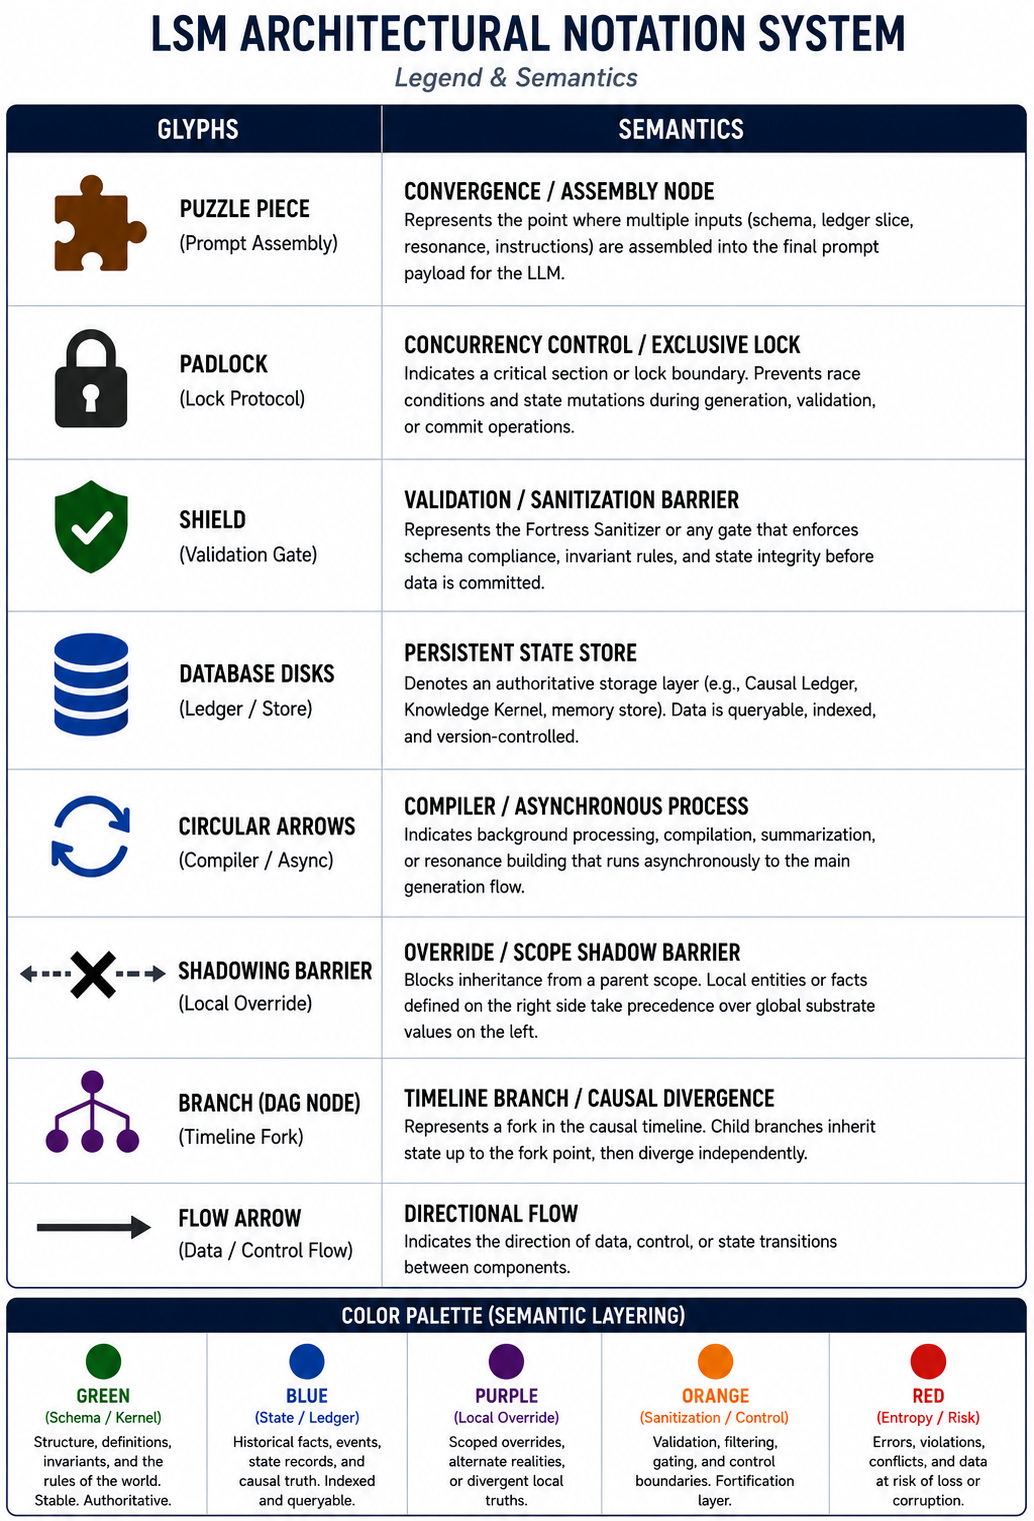
\includegraphics[width=0.94\textwidth]{images/fig_notation.png}
    \caption{The LSM Architectural Notation. Operational glyphs encode system behavior (e.g., the Puzzle Piece denotes modular prompt assembly, whereas the Shadowing 'X' denotes scoped data masking). Colors are strictly mapped to data topology (Green for Schema, Blue for State, Orange for Sanitization, Red for Entropy).}
    \label{fig:notation}
\end{figure}



\newpage
% -------------------
% Appendix D - Glossary of Concepts
% -------------------
\section{Glossary of Concepts}
\label{app:glossary}

\begin{description}
    \item[Asymmetric Co-Creation] \label{def:asymmetric}
    A design paradigm where the labor of storytelling is divided by substrate: the human operator (Director) governs the absolute ontological state, while the Large Language Model (LLM) is relegated to rendering validated prose within those constraints.

    \item[Axiomatic Investment] \label{def:axiom}
    The upfront labor required to define schemas, entity properties, and world rules; an engineering trade-off that replaces the friction of "Contextual Amnesia" with the benefit of long-term narrative stability.

    \item[Bounded Stochasticity] \label{def:bounded}
    The ability to permit high-temperature, highly creative probabilistic generation because deterministic software wrappers and strict operational locks prevent generative errors from corrupting the underlying state machine.

    \item[Causal Ledger] \label{def:ledger}
    An authoritative record of sequential turns, stored as a structured array of JSON objects. Unlike a flat transcript, the ledger is computationally queryable and supports non-linear mutation through "Causal Revisionism."

    \item[Causal Revisionism] \label{def:surgery}
    The formal algebra of timeline editing (insert, delete, split, merge, fork) that preserves narrative integrity by mechanically re-indexing the "Master Clock" and chapter boundaries.

    \item[Compounding Narrative Returns] \label{def:compound}
    A property of state-rigorous systems where the simulation becomes texturally richer and more accurate as turn counts increase, due to the continuous accumulation and refinement of resonance layers.

    \item[Contextual Amnesia] \label{def:amnesia}
    A structural failure mode in state-anemic systems where established narrative facts become unavailable or diluted at generation time due to context window saturation or attention decay.

    \item[Epistemic Agency] \label{def:epistemic}
    Power exercised by the human operator through the understanding, management, and forensic auditing of the system’s state, rather than through simple branching-path choices.

    \item[Fault-Tolerant Narrative Processing] \label{def:fortress}
    A deterministic I/O pipeline (The Fortress Sanitizer) that intercepts, repairs, and validates probabilistic LLM outputs before permitting them to touch the Causal Ledger.

    \item[Ledger Lock Protocol] \label{def:lock}
    A concurrency safeguard that physically disables state mutation in the user interface while a generative commit is in flight, preventing "Ontological Race Conditions."

    \item[Master Clock] \label{def:mclock}
    A sequential integer index assigned by the engine to every ledger entry, serving as the relative temporal coordinate system for the timeline, independent of LLM hallucinations.

    \item[Narrative Kernel] \label{def:kernel}
    The declarative T-Zero schema (e.g., \texttt{setup.json}) establishing the baseline rules, entity definitions, tone, and campaign goals before a simulation begins.

    \item[Language State Machine (LSM)] \label{def:nsm}
    A software architecture that decouples absolute world state from generative prose, treating the LLM as an untrusted rendering engine gated by deterministic logic.

    \item[Non-Destructive Orchestration] \label{def:ndo}
    The design principle requiring that all timeline revisions be explicit, named state transitions, ensuring that the causal path remains forensically auditable.

    \item[Ontological Agent] \label{def:agent}
    The role of the human operator in an LSM architecture, characterized by governing world rules and auditing memory rather than simply typing conversational prompts.

    \item[Ontological Anchoring] \label{def:anchoring}
    The process of binding generative prose to deterministic state objects (Master Clocks, Schemas, Inventory Pills). This ensures that even if the prose engine diverges, the "anchor" of reality remains fixed in the ledger.

    \item[Ontological Resonance Layers] \label{def:resonance}
    Tiered, compiled memory (Plot and Entity ledgers) extracted from the history and strategically injected into prompts to provide high-fidelity recall without context bloat.

    \item[Prequel Shadowing] \label{def:shadow}
    A "Local Override" pattern where a thread-specific entity profile takes precedence over a global profile, allowing for time-travel or flashback scenarios without corrupting the universal canon.

    \item[Prose Engine] \label{def:prose}
    The hybrid component comprising the probabilistic Large Language Model and its deterministic "Narration Adapter."

    \item[Safeguarded Divergence] \label{def:safeguard}
    Creative or chaotic variance generated by the LLM that is isolated in volatile memory until it survives sanitization gates and human approval.

    \item[State-Anemic] \label{def:anemic}
    An architecture (typical of chatbots) where world state is derived strictly from a linear transcript of prose, leading to fragility and amnesia.

    \item[State-Rigorous] \label{def:rigorous}
    An architecture where authoritative truth lives in externalized, queryable databases, ensuring that reality is durable regardless of prompt length or model drift.

    \item[Substrate Scoping] \label{def:substrate}
    The ruleset governing the merging of local thread data and global universe data during prompt assembly.

    \item[Unsafe Probabilistic Coprocessor] \label{def:coprocessor}
    The demoted role of the Large Language Model in an LSM architecture; it is treated as a high-performance but untrusted component that calculates probabilities rather than absolute truths.

\end{description}
\end{document}
